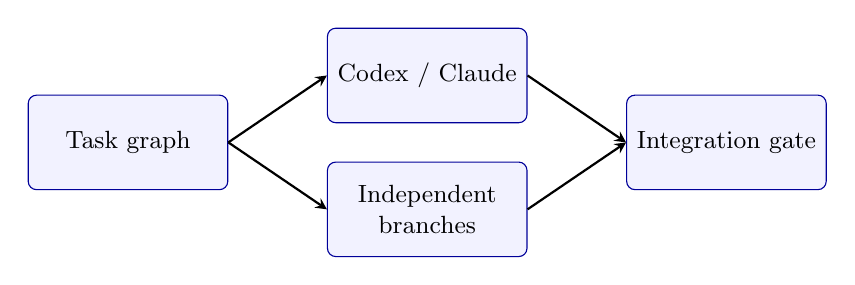
\begin{tikzpicture}[nodebox/.style={draw=blue!60!black,fill=blue!5,rounded corners=3pt,minimum height=12mm,text width=23mm,align=center,font=\small},>=stealth]
\node[nodebox] (n0) at (0.00,0.00) {Task graph};
\node[nodebox] (n1) at (3.80,0.85) {Codex / Claude};
\node[nodebox] (n2) at (3.80,-0.85) {Independent branches};
\node[nodebox] (n3) at (7.60,0.00) {Integration gate};
\draw[->,thick] (n0.east) -- (n1.west);
\draw[->,thick] (n0.east) -- (n2.west);
\draw[->,thick] (n1.east) -- (n3.west);
\draw[->,thick] (n2.east) -- (n3.west);
\end{tikzpicture}
